\colorlet{chaptergrey}{red!60!yellow!30!}
%\renewcommand*\sectfont{\color{orange}}

\chapter[Kinematic misalignment]{Kinematic misalignment}
\label{ch:kin_mis}
\vspace{-5.25in}
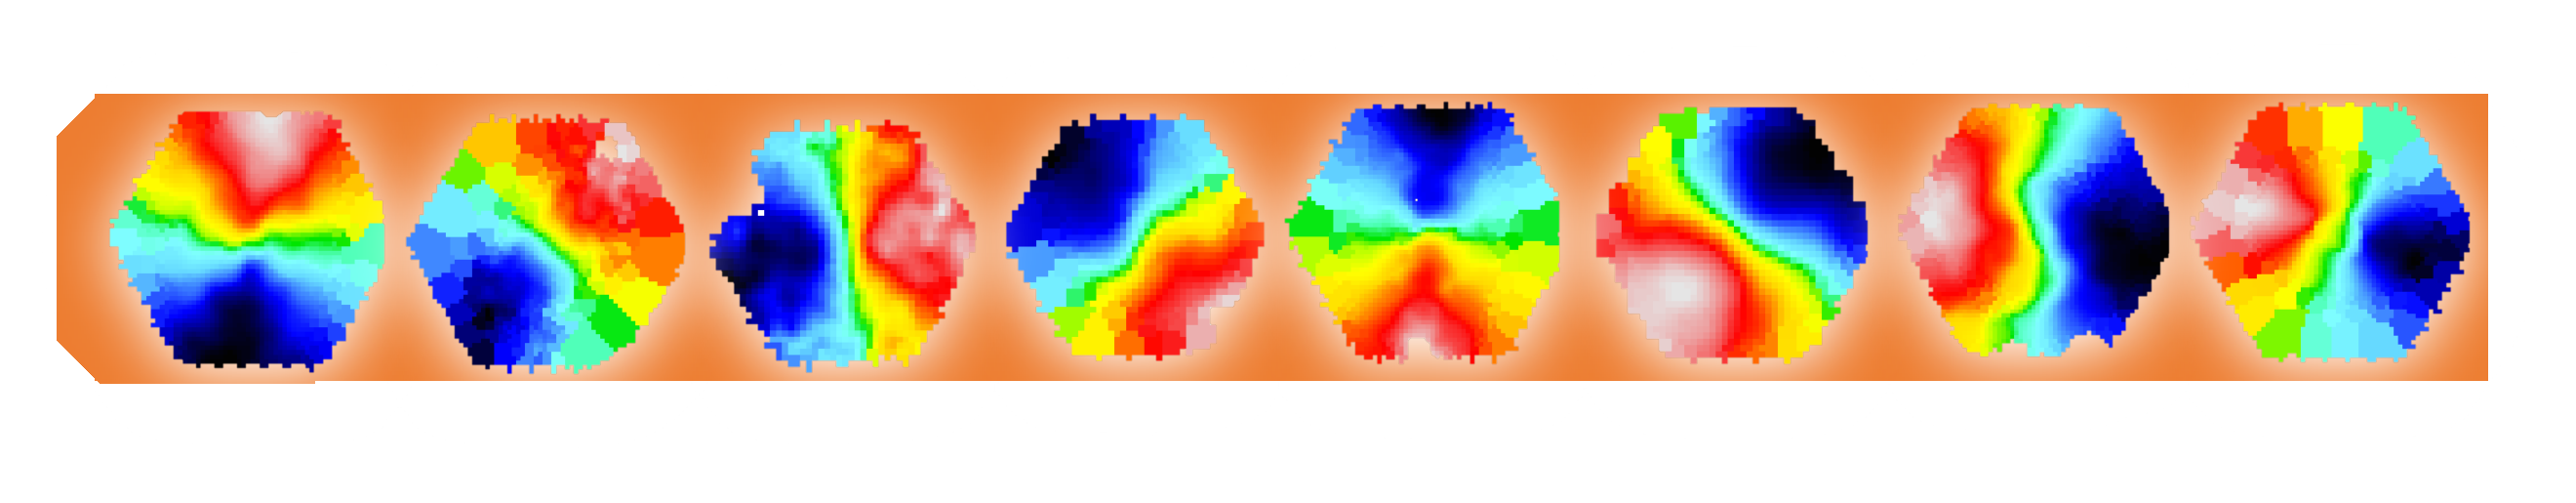
\includegraphics[height=1.39in]{thesis/latex/misalignment_intro/kin_mis_chapter_heading.pdf}
\vspace{3in}

\epigraph{This chapter is partially based on Duckworth, Tojeiro, Kraljic, Sgr\'o, Wild, Weijmans, Lacerna and Drory, in MNRAS, 448, Issue 1, 2019 and Duckworth, Tojeiro and Kraljic, in MNRAS 492, Issue 2, 2020. Here, we introduce kinematic misalignment.}

\section{Introduction}
Unlike single-fibre galaxy surveys such as SDSS which only obtain spectra from the central $\sim 3 ''$ of a target galaxy, integral field unit (IFU) observations enable spatially resolved spectral measurements up-to several effective radii (\re) across the faces of nearby galaxies. From these spectra, we can simultaneously extract kinematics of stars and gas, while obtaining absorption line strengths which provide radial gradients of gas phase metallicity and stellar population age.

\red{Go more in depth about angular momentum and link to kinematic misalignment here?} The ability to characterise the rotation of stars and ionized gas is a useful indicator of the recent interaction history of a galaxy. Assuming gas that has cooled from stellar mass loss to be kinematically aligned with the original stars, an offset between the rotation of stars and ionized gas is indicative of external gas origin \citep[see][]{sarzi2006,davis2011a}. 

\red{Expand on this and link to individual sections} Previous work has focused on the gas content in early-type galaxies (ETGs) and the fraction of which that are significantly kinematically misaligned (i.e. global position angle between rotational directions of gas and stars is greater than 30$^{\circ}$; see \S\ref{sec:kin_mis}) indicating external influence (see. \citet{davis2011a} identify that approximately 36\% of fast-rotating ETGs are kinematically misaligned within the volume-limited sample of ATLAS\textsuperscript{3D} \citep{atlas3d}. 

This can also be used to constrain the time-scales of misalignment. \citet{davis2016} utilise a toy model to propose that misaligned gas could relax gradually over time-scales of 1-5 Gyr. A faster time-scale of relaxation would require merger rates of $\approx 5$ Gyr\textsuperscript{-1} and hence is disfavoured. The interplay between the strength and persistence of the gas in-flow and the re-aligning torque of the stellar component dictates the exact time-scale of misalignment for an individual galaxy. The strength of a galaxy's stellar torque scales as a function of radius, with the central component of a galaxy re-aligning on a quicker time-scale than the outer regions. \red{We investigate this further in chapter...}

The persistence of misalignment has also been considered in numerical simulations. \citet{vdvoort2015} consider the evolution of a misaligned gas disc formed from a merger which removes most of the original disc. During re-accretion of the cold gas, the misaligned disc persists for approximately 2 Gyr before the gas-star rotation angle falls below 20$^{\circ}$. The sustainment of this misalignment is due to continued gas accretion for approximately 1.5 Gyr before its rate falls and the gas can realign with the stellar component on approximately six dynamical time-scales. \red{Should this be included here or in motivation for chapter 'timescales for misalignment'}

IFU observations are costly, and such detailed information has often come at the cost of total galaxies observed. For example, in the last 10 years ATLAS\textsuperscript{3D} and \red{CALIFA} \citep{califa} observed 260 and 667 galaxies respectively with various selection criteria. 

\red{Rewrite this sentence?} At the present-time, however, there are two large-scale IFU surveys which could provide a sample large enough for a statistically significant characterisation with respect to halo assembly and environment and to constrain relaxation timescales. The Sydney-AAO Multi-object Integral field spectrograph survey \citep[SAMI;][]{croom2012,bryant2015} will map $\sim$3400 galaxies in the local universe ($z < 0.12$) across a large range of environments in the GAMA footprint. In parallel, the Mapping Nearby Galaxies at Apache Point \citep[MaNGA;][]{bundy2015,blanton2017} survey will map $\sim$10000 galaxies up to $z = 0.15$, with the aim of creating a sample with near flat number density distribution in absolute $i$-band magnitude and stellar mass. In this Chapter, we introduce the methodology of defining kinematic misalignment in the context of the MaNGA survey. \red{In Chapter X, we determine the merger rate and relaxation timescales for ETGs through comparison of the observational misalignment fraction in MaNGA to simulated in IllustrisTNG. In Chapter Y, we investigate an unusual sub-sample of LTGs that appear to have kinematically decoupled stellar and gas components through comparison of MaNGA to IllustrisTNG. In Chapter Z, we investigate the relationship between kinematic misalignment in galaxies and their large-scale environment, in the context of halo assembly.}

\section{MaNGA}
Set to complete in 2020, the MaNGA survey is designed to investigate the internal structure of $\sim$10000 galaxies in the nearby Universe. By design, the complete sample is unbiased towards morphology, inclination and colour and provides a near flat distribution in stellar mass. 

MaNGA is one of three programs in the fourth generation of the Sloan Digital Sky Survey (SDSS-IV) which enables detailed kinematics through integral field unit (IFU) spectroscopy. MaNGA uses the SDSS 2.5 metre telescope in spectroscopic mode \citep{gunn2006} with the two dual-channel BOSS spectrographs \citep{smee2013} and the MaNGA IFUs \citep{drory2015}. MaNGA provides spatial resolution on kpc scales (2'' diameter fibres) while covering 3600-10300$\mathrm{\mathring{A}}$ in wavelength with a resolving power that varies from R$\sim$1400 at 4000$\mathrm{\mathring{A}}$ to R$\sim$2600 at 9000$\mathrm{\mathring{A}}$. 

MaNGA observations use SDSS style plates, where bundles of optical fibres are plugged into the plate corresponding to the position of the target galaxy in the observational field. A dithered pattern is employed for each target field (plate), which simultaneously observes galaxies through 17 fibre-bundles of 5 distinct sizes. Any incomplete data release of MaNGA should therefore be unbiased with respect to IFU sizes and hence a reasonable representation of the final sample scheduled to be complete in 2020.

The majority of observations contribute to one of the three main subsets: the Primary sample, the Secondary sample and the Colour-Enhanced supplement. All sub-samples observe galaxies to a minimum of $\sim 1.5$ effective radii ($\mathrm{R_{e}}$) with the Secondary sample increasing this minimum to $\sim 2.5 \mathrm{R_{e}}$. The Colour-Enhanced supplement fills in gaps of the colour-magnitude diagram leading to an approximately flat distribution of stellar mass. A full description of the MaNGA observing strategy is given in \citet{law2015obs,yan2016obs}. The raw observations are processed by the MaNGA Data Reduction Pipeline (DRP) as described in \citet{law2016drp, yan2016spec}. The fibre flux and inverse variance is extracted from each exposure, which are then wavelength calibrated, flat-fielded and sky subtracted.

MaNGA releases data periodically in the form of MaNGA Product Launches (MPL), both increasing the number of observed galaxies and updating the data processing. In the following chapters we use data from MPL-6 and MPL-8 referring to the sixth and eighth Product Launches.
% Include a figure showing the distribution of NSA, MaNGA targets, MPL-6 and MPL-8.
% Also include figure of bundle sizes?

\section{Velocity fields}
The MaNGA Data Analysis Pipeline \citep[DAP][]{westfall2019,belfiore2019} provides science-ready processed data for MaNGA observations. Some example outputs include; spaxel-by-spaxel coordinate information based on the isophotal ellipticities from the NASA-Sloan Atlas, S/N measurements, binned spectra, stellar kinematics and stellar-continuum models, emission-line properties and models, and spectral-index measurements. Kinematics are easily accessible as 2D maps which we use for stellar and gas velocity fields in the following analysis. A complete discussion can be found in \citet{westfall2019,belfiore2019}, however we will summarise the key points concerning stellar and gas velocity fields here.

The DAP extracts stellar kinematics using the Penalised Pixel-Fitting (pPXF) method \citep{cappellari2004,cappellari2017}. The DAP fits the stellar continuum of each spaxel to extract the line of sight velocity dispersion and then fits the absorption-line spectra from a set of 49 clusters of stellar spectra from the MILES stellar library \citep{sanchez2006,falcon2011}. Before extraction of the mean stellar velocity, the spectra are spatially Voronoi binned to $g$-band \textit{S/N} $\sim$ 10, excluding any individual spectrum with a $g$-band \textit{S/N} < 1 \citep{cappellari2003}. This approach is geared towards stellar kinematics as the spatial binning is applied to the continuum \textit{S/N}, however, we note that unbinned and Voronoi binned velocity maps produce similar results. 

Ionized gas kinematics are extracted by the DAP through fitting a Gaussian to the H$\alpha$-6564 emission line, relative to the input redshift for the galaxy. This velocity is representative for all ionized gas, since the parameters for each Gaussian fit to each emission line are tied during the fitting process. These velocities are also binned spatially by the Voronoi bins of the stellar continuum. 

\section{Kinematic misalignment} \label{sec:kin_mis}
We estimate the two dimensional global position angle (PA) of the stellar and H$\alpha$ gas velocity fields using the \texttt{FIT\_KINEMATIC\_PA} routine outlined in Appendix C of \citet{krajnovic2006}. By default this finds the angle corresponding to the bisecting line which has greatest velocity change along it (i.e. the angle of peak rotational velocity). We choose this angle to be found from sampling at 180 equally spaced steps. This is measured counter-clockwise from the north axis, however, it does not discriminate between the blueshifted and redshifted side since it is only defined up to 180$^{\circ}$. As a result, velocity fields with a difference of 180$^{\circ}$ PA would appear to be aligned. To solve this we identify the direction of rotation and re-assign a consistent PA: defined as the axis of rotation approximately 90$^{\circ}$ clockwise from the blueshifted side. This angle now spans 360$^{\circ}$ allowing an automatic detection of misaligned gas and stellar components. The offset angle between kinematic components is defined as: 
\begin{equation} \label{eq:delPA}
\mathrm{\Delta PA = |PA_{stellar} - PA_{H\alpha}|. }
\end{equation}
We define galaxies with $\Delta$PA > 30$^{\circ}$ to be significantly kinematically misaligned. An example of an aligned and a misaligned galaxy is shown in Figure \ref{fig:cutout_wIFU}. 

\begin{figure*}
    \centering
	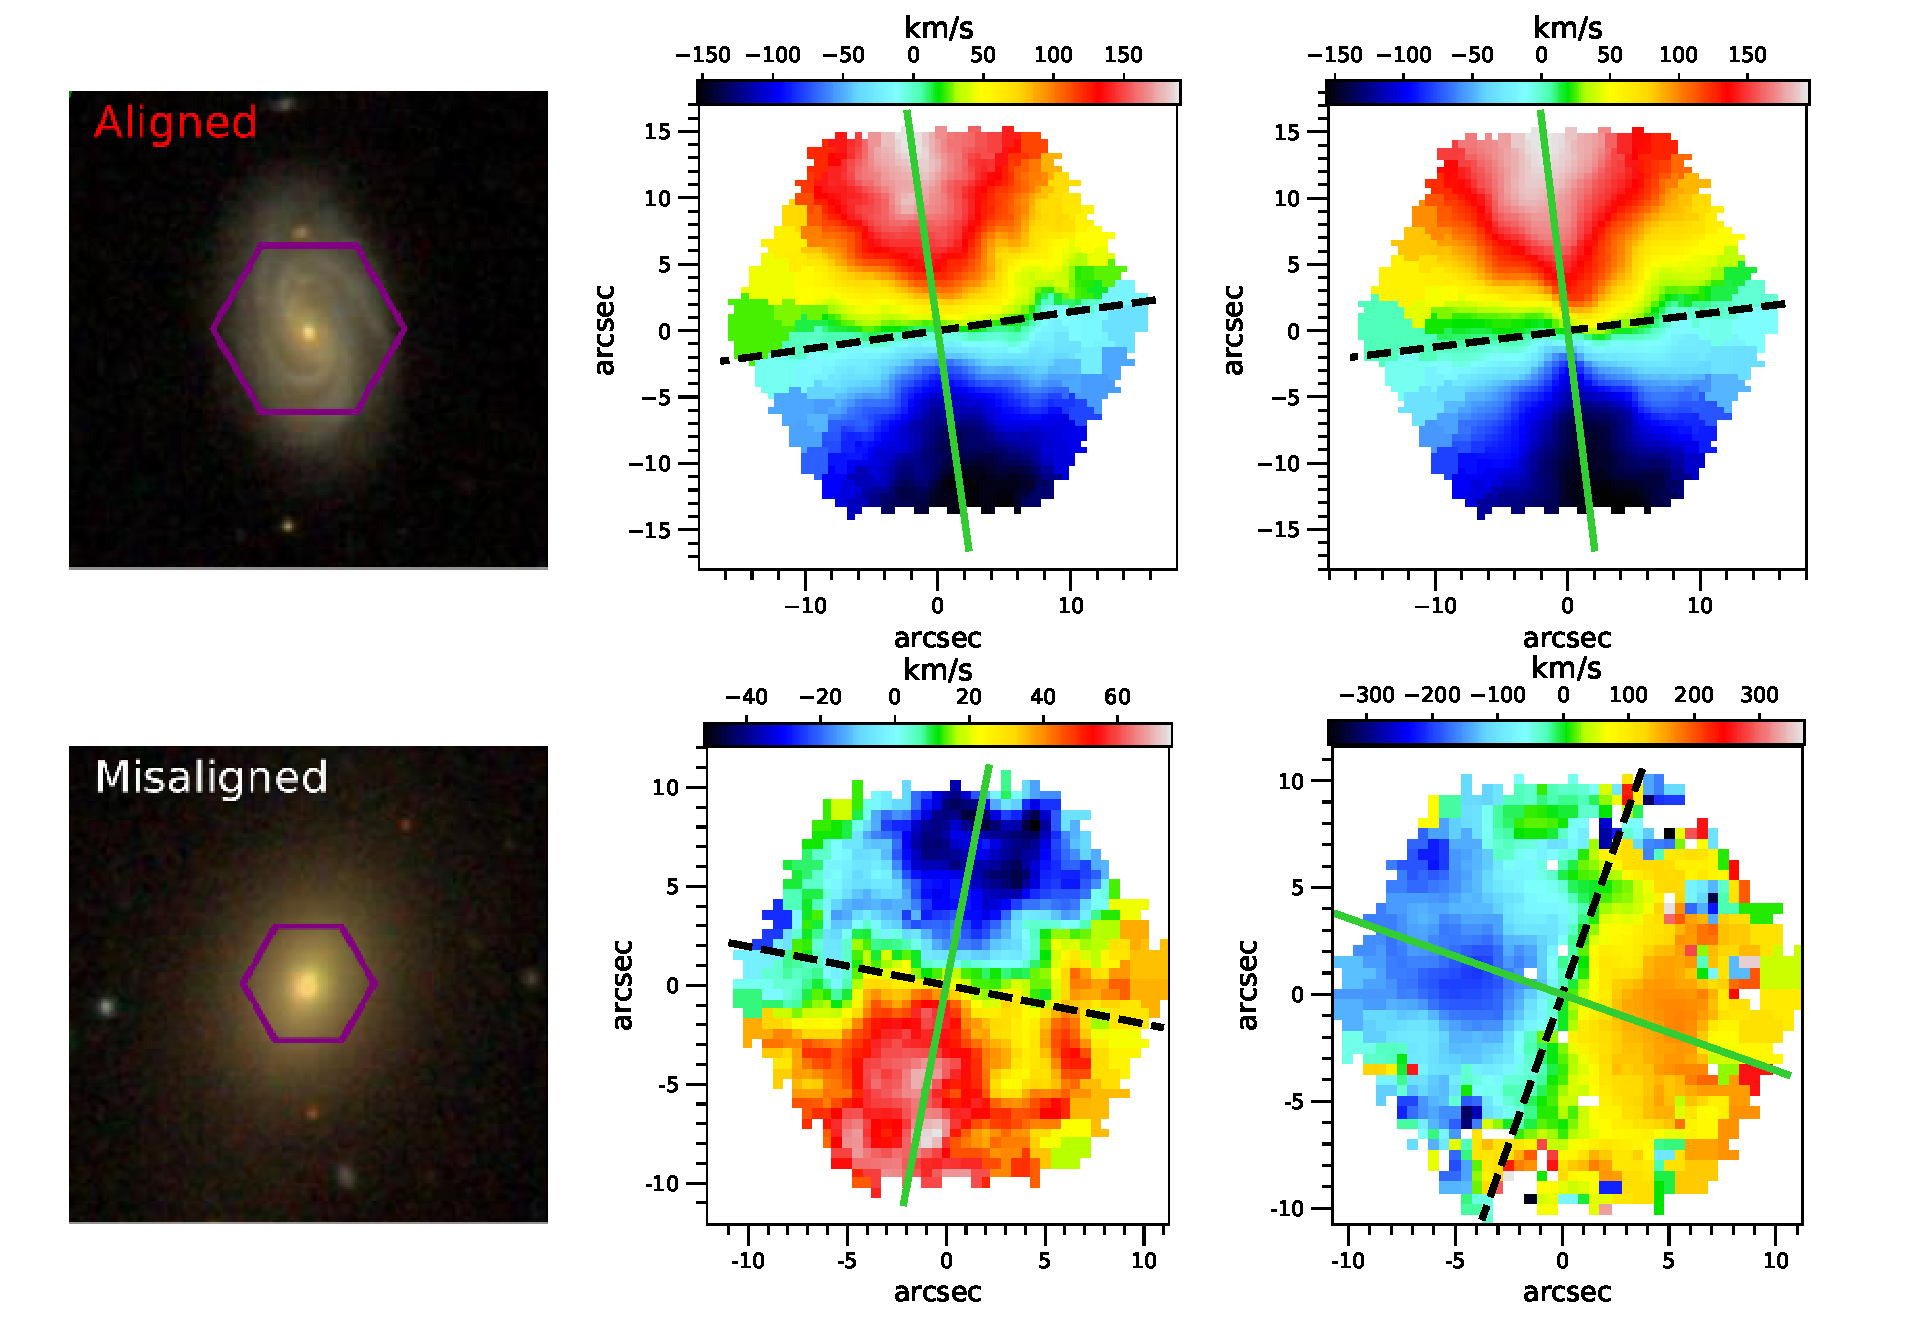
\includegraphics[width=0.8\linewidth]{thesis/latex/misalignment_intro/cutout_wIFU_revised.pdf}
    \caption[Examples of a kinematically aligned (top) and misaligned (bottom) galaxy defined by $\Delta$PA.]{Examples of a kinematically aligned (top) and misaligned (bottom) galaxy defined by $\Delta$PA. From left to right, the panels show (i) the original SDSS cutout of surrounding field with the MaNGA IFU footprint overlaid in purple, (ii) stellar velocity field and (iii) $H\alpha$ (gas) velocity field. The velocity fields are marked by a defined PA (green solid line) and axis of rotation (black dashed line). The galaxy in the bottom row is misaligned due to it having $\Delta$PA > 30$^{\circ}$. The colour-bars represent the velocity fields in km/s and the galaxies are orientated so that up corresponds to North and right to East.}
    \label{fig:cutout_wIFU}
\end{figure*}

To improve the reliability of the PA fit, we apply a few additional filters to the velocity fields. While foreground stars are flagged within observations, background/small neighbouring galaxies can remain within the IFU footprint. This is a problem for fitting a global position angle since it naturally interprets other material as part of the target galaxy's observation and interpolates between the regions. We remove all disconnected regions smaller than $10\%$ of the target galaxy's footprint. In addition we sigma clip the velocity field and remove all spectral pixels (spaxels) above a $3\sigma$ threshold.

Our choice to take $\Delta$PA > 30$^{\circ}$ as significantly kinematically misaligned is a conservative selection to ensure we are selecting galaxies undergoing external interaction. There is evidence to suggest that accretion drives misalignment past $\Delta$PA = 30$^{\circ}$. \citet{lagos2015} found that using solely galaxy mergers as the source for misaligned cold gas only predicts 2\% of ETGs to have $\Delta$PA > 30$^{\circ}$ using GALFORM, in comparison with the misaligned field ETG fraction found in ATLAS\textsuperscript{3D} of 42 $\pm$ 6\%  \citep{davis2011a}. This puts a lower level of importance on gas accretion. Our choice can be justified as follows. Firstly, we are using ionized gas as a proxy for the distribution and accretion of cold gas. \citet{davis2011a} find that the typical difference between the PAs of cold gas (CO) and ionized gas can be described by a Gaussian distribution centred on 0 with a standard deviation of 15$^{\circ}$ for 38 CO bright galaxies in ATLAS\textsuperscript{3D}. While indicating ionized gas is a reasonable estimator for cold gas, splitting $\Delta$PA = 30$^{\circ}$ accounts for the scatter in this relationship. Secondly, this should avoid spurious misalignments arising from errors in the fit of $\Delta$PA. While our model errors are low, they are likely an underestimation since they do not include more complex motions. However, selecting a lower split in $\Delta$PA would only be affected by the increased likelihood of internal processes being dominant, rather than the inaccuracy of fitting. Any threshold in $\Delta$PA becomes a trade off between sample size and contamination probability. Altering our cut in $\Delta$PA to be 20$^{\circ}$, 40$^{\circ}$ or similar does not change any of the conclusions drawn in this chapter.

\subsection{Error estimation}
It is an important point to constrain the errors of our PA fits, so we can reliably trust cuts in $\Delta$PA to select galaxies which are significantly kinematically misaligned and hence have had external interaction. Here, we construct two component model velocity maps for each stellar and gas component of every MPL-6 observation in order to estimate typical errors on $\Delta$PA from \texttt{FIT\_KINEMATIC\_PA} for the MaNGA sample. \red{MPL-6 corresponds to a total of 4633 unique galaxy observations.}

Errors using the \texttt{FIT\_KINEMATIC\_PA} routine have been previously estimated for molecular gas velocity fields in ATLAS\textsuperscript{3D} \citep{davis2011a}. Model velocity fields with a known PA were constructed using an empirical galaxy rotation curve and combined with Gaussian noise matched to the signal-to-noise ratio of the data. A typical scatter of $\approx10^{\circ}$ was found due to varying inclination and angular resolution for the velocity fields.

\subsubsection{Circular velocity}
To find the typical error on $\Delta$PA for galaxies in MaNGA, we create model velocity maps for both the stellar and gas components of each MPL-6 observation. In each instance the basic construction of the model follows Section 4 of \citet{krajnovic2006}. Each velocity field comprises of a two-component Hernquist potential which provides a basic circular velocity given by,
\begin{equation}
\mathrm{V_c = \frac{\sqrt{GMr}}{r+r_0}}
\end{equation}
where $G$ is the gravitational constant, $M$ is the total mass and $r_0$ is the core radius of each component respectively \citep{hernquist1990}. We use a two-component model to include the relative strengths of both disc and bulge each with distinct effective radii, $R_e$. We fix $r_0$ to be 5 and 15 (units: $arcsec$) and $\sqrt{GM}$ to be 850 and 1500 (units: $km s^{-1} arcsec^{1/2}) $ for the bulge and disc components respectively. These individual components are light weighted by model sersic flux profiles according to,
\begin{equation}
\mathrm{I(r) = I_0 e^{-\left(\frac{R}{R_e}\right)^{n_s}}}
\end{equation}
where $I_{0}$ is the peak flux and $n_s$ is the sersic index which is set to 1 and 4 for the disc and spheroidal components respectively. Since we do not have bulge-disc decompositions, we lack individual effective radii for both the bulge and disc components. Instead, we set the bulge and disc effective radii to be 0.5$R_e$ and 1.5$R_e$, where $R_e$ is the effective radius estimated by an elliptical petrosian fit taken from the NSA targeting catalogue. 

\subsubsection{Calibration}
For each MaNGA galaxy a basic velocity field model is constructed using this template. The axes of the model velocity field are then scaled according to the inclination, $i$, which is estimated from the $b/a$ ratio taken from the NSA catalogue and is also used to scale the fraction of rotational velocity along the line-of-sight. The velocity field for each component, ($j=bulge,disc$), in polar coordinates $(r,\phi)$ is then described by,
\begin{equation}
\mathrm{V(r,\phi) = \frac{I_{j}(r)}{I_{tot}(r)}V_{c}(r)\cos(\phi+\theta_{j})\sin(i)}
\end{equation}
where $\theta_j$ is the input kinematic position angle. We set $\theta_{bulge} = \theta_{disc}$ for simplicity, however, we do note that galaxies with more complex orbital motions may increase the typical error. The position angle for both bulge and disc is simply taken to be the opening angle of the galaxy (direction of major axis taken from NSA catalogue). 

In order to imitate a MaNGA observation, the model velocity field is sampled at the spatial resolution of the corresponding IFU bundle and projected into the original shape of the actual observation for H$\alpha$ and stellar maps respectively. Gaussian noise is drawn for each spaxel from a normal distribution with the standard deviation taken from the errors on the actual observation. In addition, these model velocity fields are then Voronoi binned to match the original observation.

Example stellar and H$\alpha$ velocity fields generated from these models are shown in Figure \ref{fig:sim_ifu} with comparison to the actual observation. As expected, the model velocity fields frequently recreate observations well but struggle to encompass more complex motion. For this reason, our models should make a reasonable prediction on the typical $\Delta$PA errors intrinsic to MaNGA observations.

\begin{figure}
    \centering
	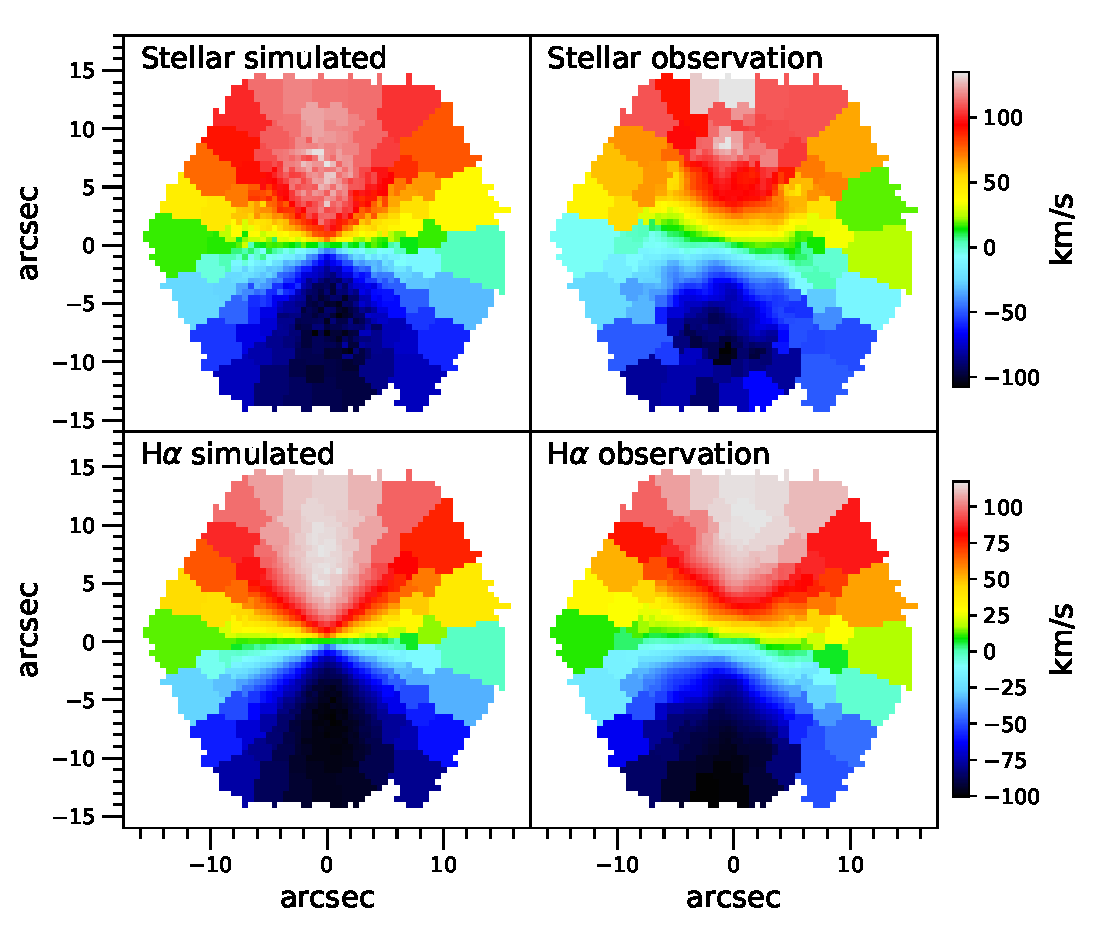
\includegraphics[width=0.7\linewidth]{thesis/latex/misalignment_intro/obs_sim_IFU.pdf}
    \caption[Comparison velocity maps for simulation (left column) and observation (right column).]{Comparison velocity maps for simulation (left column) and observation (right column). Stellar (H$\alpha$) component velocity maps are shown on the top (bottom) row with the associated velocity colourbars.}
    \label{fig:sim_ifu}
\end{figure}

\subsubsection{Typical errors}
We construct model velocity fields for all non-critically flagged MPL-6 galaxies, inclusive of the $\Delta$PA sample used in this work. Figure \ref{fig:model_errors} shows the cumulative probability distribution for the range of $0-5^{\circ}$ where the majority of errors fall. We find that \texttt{FIT\_KINEMATIC\_PA} gives a typical combined (stellar and gas) mean error of $1.3^{\circ}$. While this is an underestimation of true $\Delta$PA errors for a sample of galaxies including those with more complex velocity fields, it is indicative that selecting a cut at $\Delta$PA = 30$^{\circ}$ should be robust to identifying galaxies with external interaction. \todo{Has python version of fit kinematic pa been updated to include this?}

\begin{figure}
    \centering
	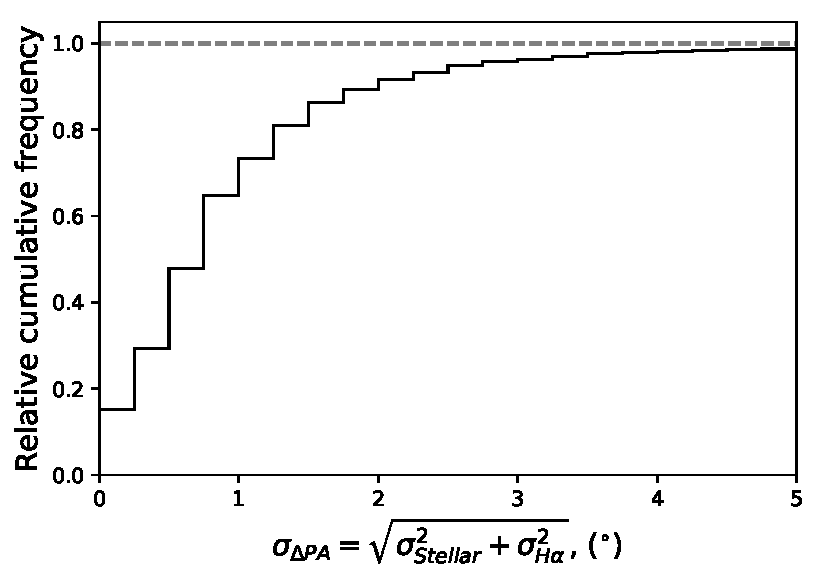
\includegraphics[width=0.6\linewidth]{thesis/latex/misalignment_intro/cumulative_model_errors.pdf}
    \caption{Cumulative histogram of errors for fitting kinematic PA to model maps for the all non-critically flagged MPL-6 galaxy observations.}
    \label{fig:model_errors}
\end{figure}

\subsection{Visual Classification}
Global position angles are only well defined for coherently rotating velocity fields. Those with a decoupling between inner and outer regions due to warps or kinematically decoupled cores (KDCs) are poorly described by global PAs. To select a clean sample of galaxies with well defined global PAs, we visually classify all of the velocity fields after pre-processing and PA fitting. Both stellar and H$\alpha$ velocity fields are characterised into 3 categories;
\begin{itemize}
    \item Dominant coherent rotation and well defined PA.
    \item Dominant coherent rotation but with more noise or more complex motion resulting in a usable PA fit but with higher typical errors. Highly inclined velocity fields with a higher likelihood of inaccurate PAs fits are included in this category. 
    \item Do not use.
\end{itemize}

Kinematic features are also identified. Both stellar and H$\alpha$ velocity fields are classified into;
\begin{itemize}
    \item Kinematically decoupled core (i.e. those with a central component that rotates in a different direction ($> 30^{\circ}$) with respect to the overall galaxy rotation).
    \item Warp (velocity field of central region is warped with respect to outskirts. This may be due to a bar, oval shaped structures in the disc (oval distortions) or accretion of fresh material with different angular momentum to the bulk rotation).
    \item Merger (ongoing merger or neighbour identified within IFU. Only those with obvious disruption are followed up in photometry).
    \item No features.
\end{itemize}
The majority of those with kinematic features have poorly defined global PAs and hence are flagged as do not use for the previous flag. The galaxies we refer to as `warped' represents a combination of galaxies with bars, oval distortions and differential rotation in the disc \citep[e.g.][]{barrera2014}. We direct the reader to \citet{stark2018} for an approach to separate the galaxies we refer to as warps. In this work, we enforce axisymmetry for our sample and hence make no use of galaxies that have significant variations in their PA as a function of radius.

For studies of quenching it may be useful to consider galaxies that have defined stellar rotation but lack coherent motion in the ionized gas. For galaxies that have usable PAs for the stellar velocity but unusable PAs for the ionized gas, we define a further classification of the gas velocity field;
\begin{itemize}
    \item Depletion (seen as empty spaxels signifying lack of gas, usually in central regions)
    \item No clear rotation (map has no clear rotation or is noise dominated)
    \item Partial rotation (partial coherent rotation in the velocity field, however there are significant regions with incoherent motion or noise domination)
    \item No clear characteristics/ No gas.
\end{itemize}
We note there is a clear overlap between the classifications for depletion and no clear rotation, since velocity fields are often a combination of these two features. 
%The total numbers for each classification in each category are summarised in Table \ref{tab:kin_class}. 
Examples of PA fits (see \S\ref{sec:def_kin_mis} for calculation) with the associated photometry for various kinematic classifications is given in Figure \ref{fig:mis_grid}. Examples of galaxies that are kinematically aligned, misaligned, have a stellar kinematically decoupled core, have a warped H$\alpha$ velocity field and have clear stellar rotation but depleted ionized gas/ no rotation are shown respectively.

\begin{figure*}
    \centering
	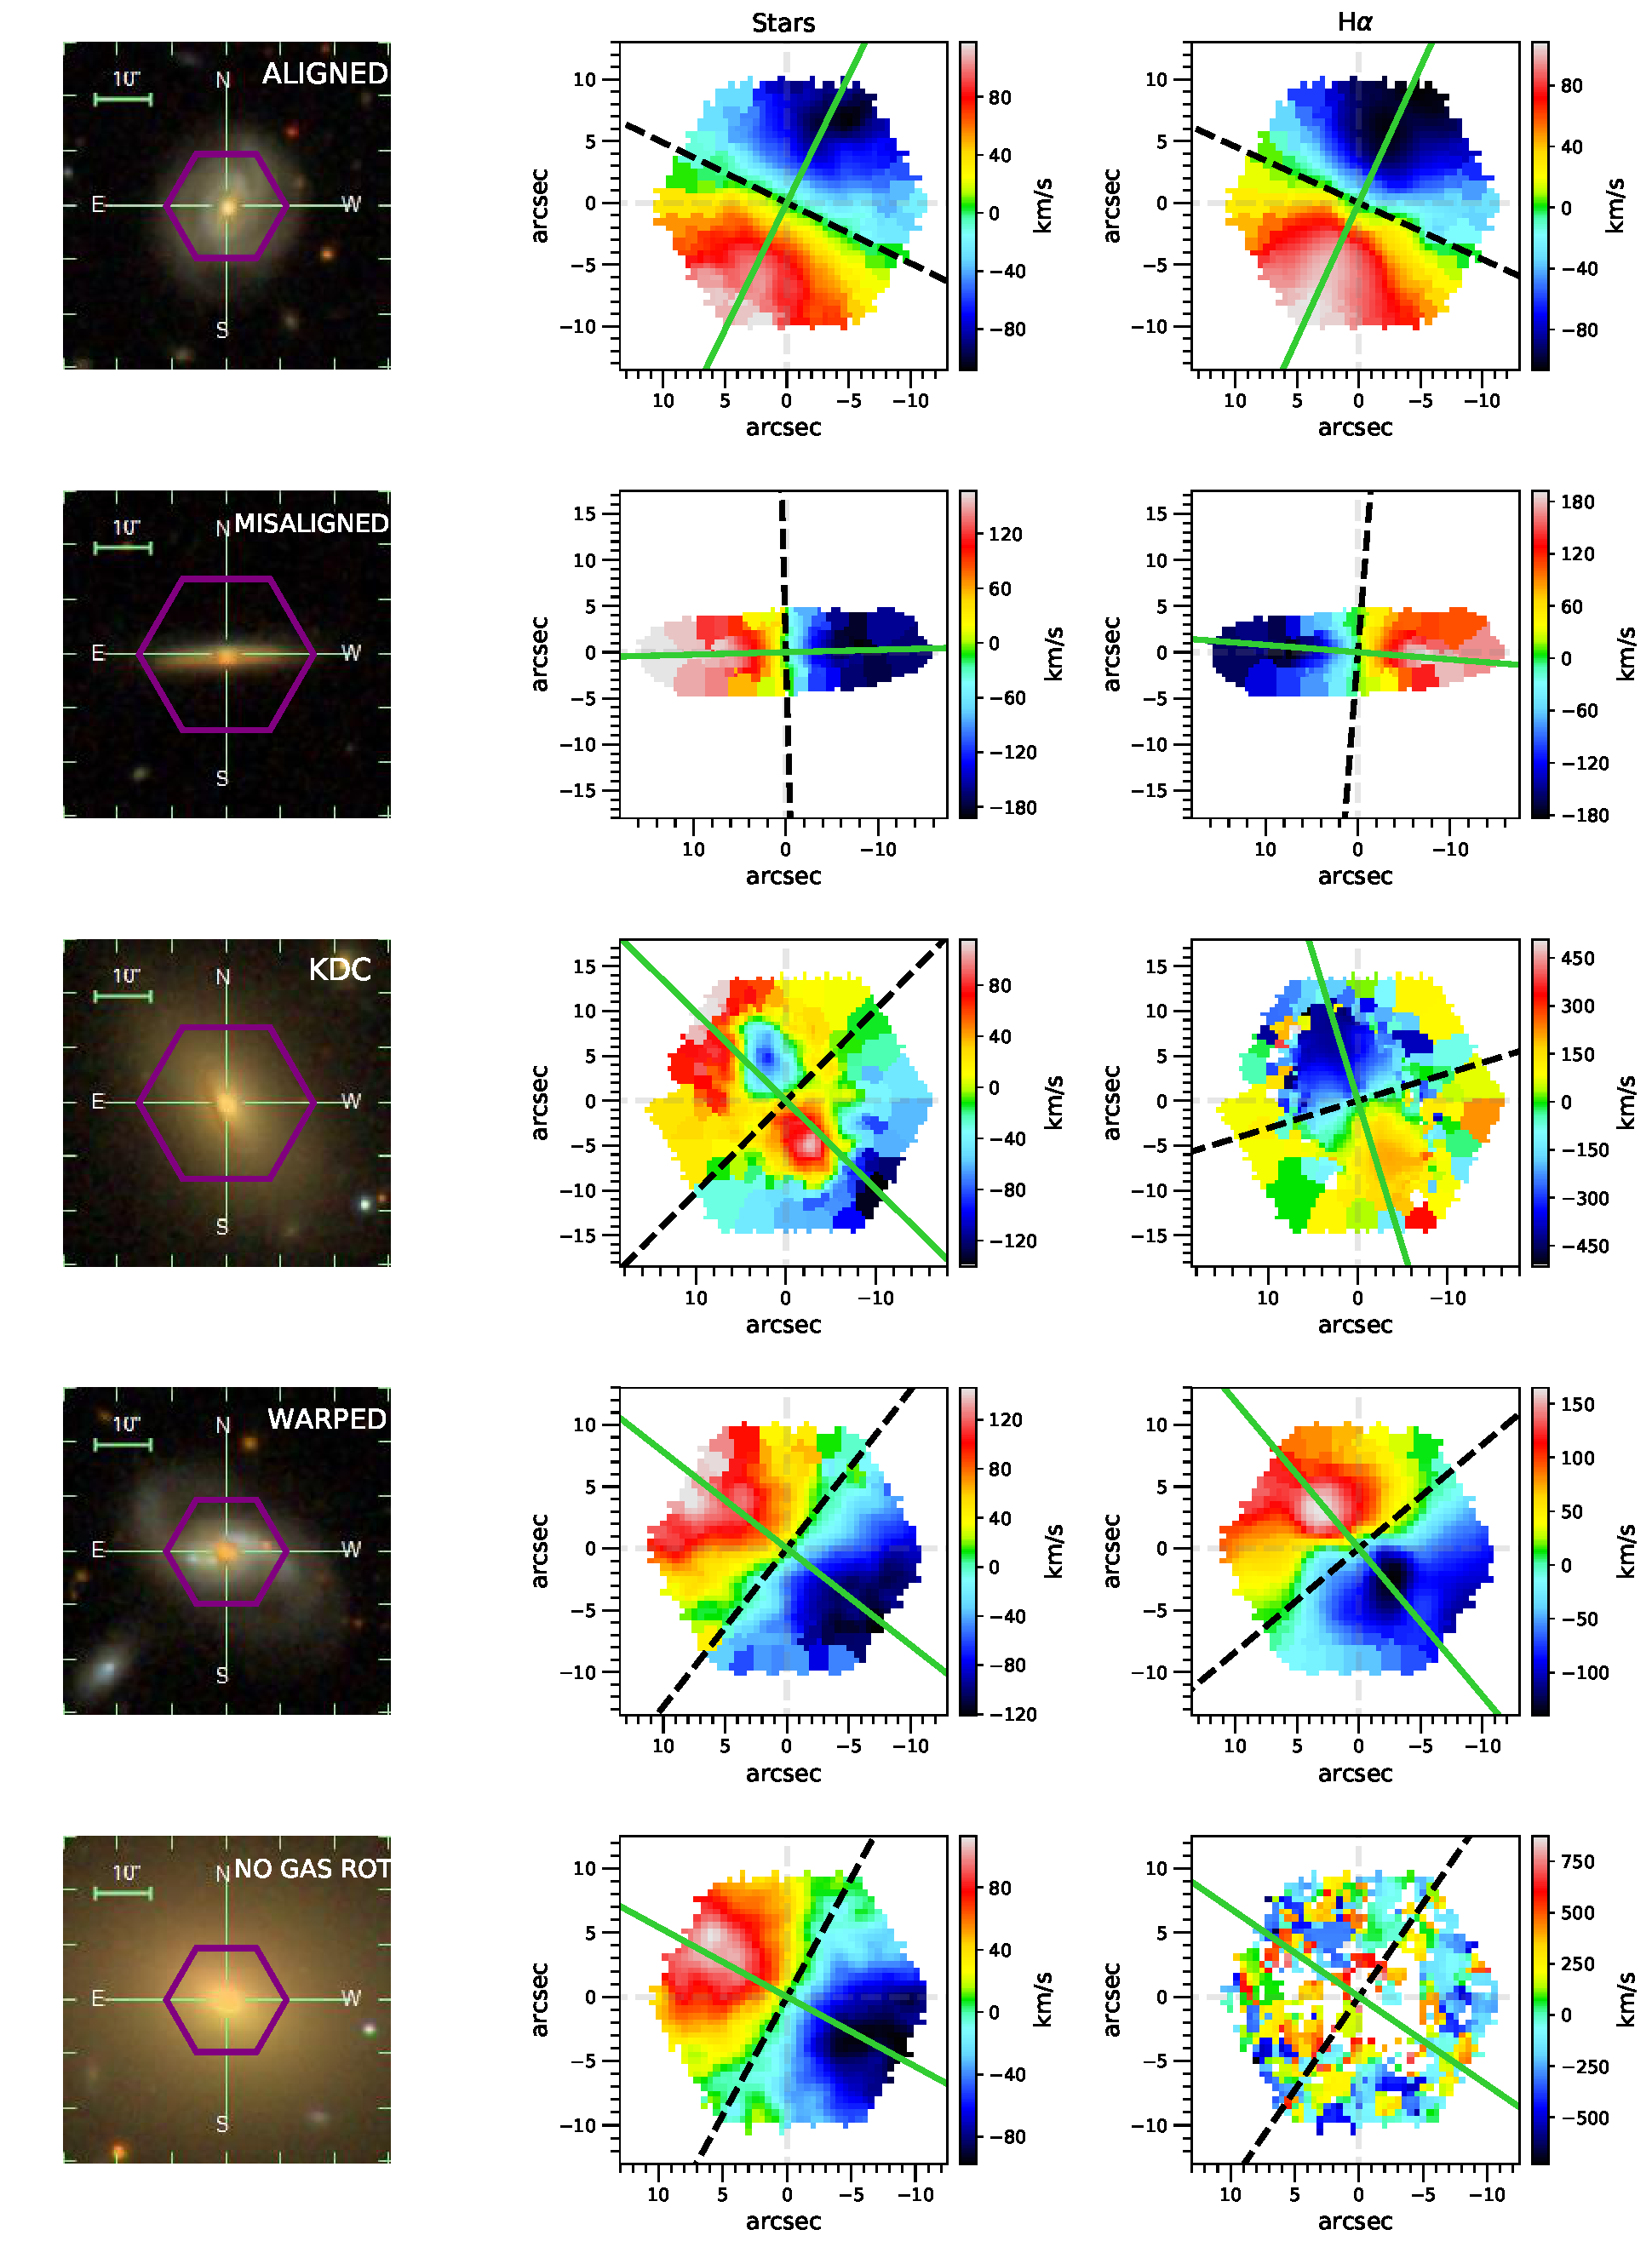
\includegraphics[width=0.93\linewidth]{thesis/latex/misalignment_intro/misalignment_grid.pdf}
    \caption{Examples of PA fits for galaxies with different kinematic classifications. For each galaxy (row), we show the photometry taken from SDSS with the MaNGA IFU observation footprint overlaid in purple (left), the stellar velocity field (middle) and the H$\alpha$ velocity field (right). The kinematic PA fits (see \S\ref{sec:def_kin_mis}) are shown on the velocity fields (green solid line) with the axis of rotation (black dotted line). The kinematic classifications from top to bottom are; (a) PLATEIFU: 7958-6101, kinematically aligned near face on; (b) PLATEIFU: 8465-12704, counter-rotating near edge on; (c) PLATEIFU: 9868-12704, with a KDC in the stellar velocity; (d) PLATEIFU: 8252-6103, with a warped H$\alpha$ velocity field with respect to the stellar; (e) PLATEIFU: 10219-6102, with a centrally depleted/missing H$\alpha$ velocity field but coherent rotation in the stellar.}
    \label{fig:mis_grid}
\end{figure*}

\red{Add subsection explaining aims and introducing next sections?}